% !TeX root = /Users/virhuiai/hlProjects/Latex-Typesetting-Hub/宏包文档翻译/tcolorbox/tcolorbox.tex

\section{Macros for Box Creation\\创建盒子的宏命令}%
\tcbset{external/prefix=external/coremacros_}%

% \include*{coremacros/tcolorboxEnv}
% \include*{coremacros/tcblowerCmd}
\include*{coremacros/tcbsetCmd}
\end{document}









\begin{docCommand}{tcbsetforeverylayer}{\marg{options}}
\begin{stripedbox}
Sets options for every following \refEnvLe{tcolorbox} inside the current \TeX\ group.
In contrast to \refComLe{tcbset}, this does also
apply to nested boxes, see \Vref{subsec:everybox}.
Technically, the \meta{options} are appended to the default values for every
tcolorbox which are applied by \refKeyLe{/tcb/reset}.\par
\tcblower
为当前\TeX\ 分组中的后续 \refEnvLe{tcolorbox} 设置选项。
与 tcbset 相比,这也适用于嵌套框,请参见 \Vref{subsec:everybox}.
从技术上讲,  \meta{options} 将附加到 \refKeyLe{/tcb/reset} 设置的 tcolorbox 的默认值。\par
\end{stripedbox}



  
You should not use this macro, if you are not completely sure that you
want to have the \meta{options} also for boxes in boxes (in boxes in boxes \ldots).

如果您不完全确定要将 \meta{options} 也用于盒子中的盒子(在盒子中的盒子中的\ldots),则不应使用此宏。
\begin{dispExample}
\tcbset{colback=green!10!white}
\tcbsetforeverylayer{colframe=red!75!black}

\begin{tcolorbox}[title=All options for this box]
这是一个tcolorbox.\par\medskip
  \begin{tcolorbox}[title=嵌套的盒子]
    注意,这个嵌套的盒子有着红色的边框,但没有绿色的背景色。
  \end{tcolorbox}
\end{tcolorbox}
\bigskip

\begin{tcolorbox}[reset]
|\tcbsetforeverylayer| 设置的选项,不受 |reset| 的影响。
\end{tcolorbox}
\end{dispExample}
\end{docCommand}
% Options given with |\tcbsetforeverylayer| survive a |reset|.


% \clearpage
\begin{docCommand}{tcbox}{\oarg{options}\marg{box content}}
  
Creates a colored box which is fitted to the width of the given \meta{box content}. 
In principle, most \meta{options} for a \refEnvLe{tcolorbox}
can be used for |\tcbox| with some restrictions. 
A |\tcbox| cannot have
a lower part and cannot be broken.

创建一个盒子, 适应给定的\meta{box content}的宽度。%
原则上, 大部分用在 \refEnvLe{tcolorbox} 上的 \meta{options},用在 |\tcbox| 上时有一些限制。%
比如,|\tcbox| 没有lower部分,也不能分页。

\begin{dispExample}
\tcbset{colframe=blue!50!black,colback=white,colupper=red!50!black,
        fonttitle=\bfseries,nobeforeafter,center title}

Text \tcbox[tcbox raise base]{你好世界}\hfill
%
\tcbox[left=0mm,right=0mm,top=0mm,bottom=0mm,boxsep=0mm,
  toptitle=0.5mm,bottomtitle=0.5mm,title=我的表格]{%
  \arrayrulecolor{blue!50!black}\renewcommand{\arraystretch}{1.2}%
  \begin{tabular}{r|c|l}
  一   & 二    & 三 \\\hline\hline
  Men   & Mice   & Lions \\\hline
  Upper & Middle & Lower
  \end{tabular}}\hfill
%
\tcbox[colback=blue!85!black,
  left=0mm,right=0mm,top=0mm,bottom=0mm,boxsep=1mm,arc=0mm,boxrule=0.5pt,
  title=我的图片]{%
  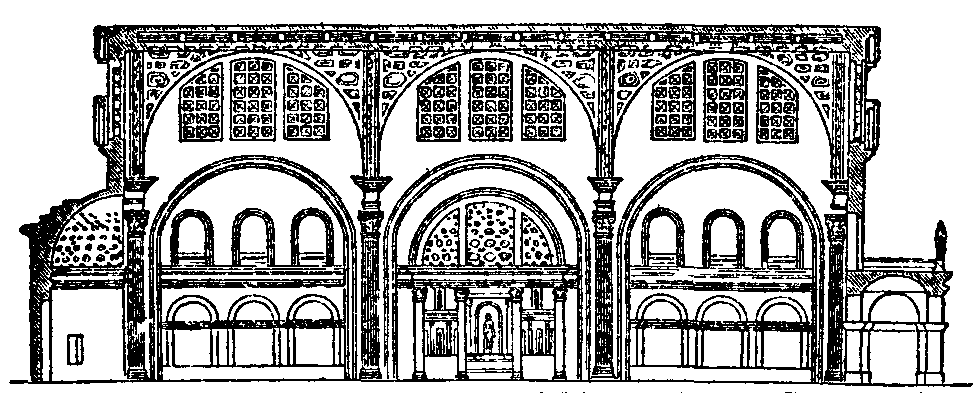
\includegraphics[width=5cm]{Basilica_5.png}}
\end{dispExample}

\begin{dispExample}
% \usepackage{tikz}
\tcbset{colframe=blue!50!black,colback=white,colupper=red!50!black,
        fonttitle=\bfseries,center title}

% 固定宽度的盒子
\begin{tcolorbox}tcolorbox中\\可以使用换行命令!\end{tcolorbox}

% 盒子的宽度自适应 (类似 hbox 、 makebox)
\tcbox{tcbox中\\换行命令\newline 无效的情况!}

% 盒子的宽度自适应 (使用 \tikzname\  node)
\tcbox[tikznode]{你好\\tikznode可以换行!}
\end{dispExample}

\end{docCommand}

% \clearpage
\begin{marker}
See \Vref{subsec:xparse_tcolorbox} and \Vref{subsec:xparse_tcbox} for more
elaborate methods to create new environments and commands.

参见 \Vref{subsec:xparse_tcolorbox} 和 \Vref{subsec:xparse_tcbox} 了解更多创建新环境和命令的方法。%详细阐述
\end{marker}

\begin{docCommand}{newtcolorbox}{\oarg{init options}\marg{name}\oarg{number}\oarg{default}\marg{options}}
  Creates a new environment \meta{name} based on \refEnvLe{tcolorbox}.
  Basically, |\newtcolorbox| operates like |\newenvironment|. This means,
  the new environment \meta{name} optionally takes \meta{number} arguments, where
  \meta{default} is the default value for the optional first argument.
  The \meta{options} are given to the underlying |tcolorbox|.
  Note that \refKeyLe{/tcb/savedelimiter} is set to the given \meta{name}
  automatically.
  The \meta{init options} allow setting up automatic numbering,
  see Section \ref{sec:initkeys} from page \pageref{sec:initkeys}.

基于\refEnv{tcolorbox}创建一个新的\meta{name}环境。%
基本上,|\newtcolorbox| 类似于 |\newenvironment|。%
% 这意味着,
新环境 \meta{name} 拥有 \meta{number} 个参数,%
其中 \meta{default} 是可选的第一个参数的默认值。%
\meta{options} 会被传递给底层的 |tcolorbox|。%
请注意 \refKeyLe{/tcb/savedelimiter} 将自动设置给 \meta{name}。%
可以在\meta{init options}中设置自动编号,%
请参阅\pageref{sec:initkeys}页的\ref{sec:initkeys}小节。


\begin{dispExample*}{sbs,lefthand ratio=0.6}
\newtcolorbox{mybox}{colback=red!5!white,
  colframe=red!75!black}

\begin{mybox}
这是我的盒子。
\end{mybox}
\end{dispExample*}

\begin{dispExample*}{sbs,lefthand ratio=0.6}
\newtcolorbox{mybox}[1]{colback=red!5!white,
  colframe=red!75!black,fonttitle=\bfseries,
  title={#1}}

\begin{mybox}{你好呀}
这是我定义的盒子,带有必选的标题参数。%
\footnote{译者发现,dispExample中定义的盒子,%
在环境外失效。}
\end{mybox}
\end{dispExample*}

\begin{dispExample*}{sbs,lefthand ratio=0.6}
\newtcolorbox{mybox}[2][]{colback=red!5!white,
  colframe=red!75!black,fonttitle=\bfseries,
  colbacktitle=red!85!black,enhanced,
attach boxed title to top center={yshift=-2mm},
  title={#2},#1}

\begin{mybox}[colback=yellow]{Hello there}
这是我定义的盒子,带有必选的标题参数和%
可选的配置参数。
\end{mybox}
\end{dispExample*}

\inputpreamblelisting{A}

\begin{tcolorbox}[breakable, title=译者对上面这个盒子的分析]
  上面由一条命令生成:

  \begin{minted}{latex}
  \inputpreamblelisting{A}
  \end{minted}

  \tcbline  

  这条命令定义为:
  \begin{minted}{latex}
  \newcommand{\inputpreamblelisting}[1]{%
  \tcbinputlisting{title=导言中的定义:,
    base example,coltitle=black,fonttitle=\itshape,titlerule=0pt,
    colbacktitle=Navy!15!ExampleBack,
    top=0mm,
    %before=\par\smallskip,%
    before skip balanced=4pt plus 2pt minus 1pt,
    after skip balanced=5pt plus 2pt minus 1pt,
    listing style=mydocumentation,
    listing only,listing file={\jobname_preamble_#1.tex}}%
  }
  \end{minted}

  \tcbline  

  可以看出代码内容来自 |\jobname_preamble_A.tex|:
  \begin{minted}{latex}
  \begin{tcbverbatimwrite}{\jobname_preamble_A.tex}
    \newtcolorbox[auto counter,number within=section]{pabox}[2][]{%
      colback=red!5!white,colframe=red!75!black,fonttitle=\bfseries,
      title=Examp.~\thetcbcounter: #2,#1}
    \end{tcbverbatimwrite}
  \end{minted}
\end{tcolorbox}


%todo dispExample 的这几个参数后面加上引用
\begin{dispExample*}{sbs,lefthand ratio=0.6}
\begin{pabox}[colback=yellow]{Hello there}
这是我的盒子,带有一一个可选参数和一个必填的带有编号的标题。
\end{pabox}
\end{dispExample*}
\end{docCommand}


\begin{docCommand}{renewtcolorbox}{\oarg{init options}\marg{name}\oarg{number}\oarg{default}\marg{options}}
  Operates like \refComLe{newtcolorbox}, but based on |\renewenvironment| instead of |\newenvironment|.
  An existing environment is redefined.

操作类似 \refComLe{newtcolorbox},但是是基于 |\renewenvironment| 而不是 |\newenvironment|。一个已存在的环境被重新定义。
\end{docCommand}


% \clearpage
\begin{docCommand}{newtcbox}{\oarg{init options}\brackets{\texttt{\textbackslash}\meta{name}}\oarg{number}\oarg{default}\marg{options}}
  Creates a new macro \texttt{\textbackslash}\meta{name} based on \refComLe{tcbox}.
  Basically, |\newtcbox| operates like |\newcommand|.
  The new macro \texttt{\textbackslash}\meta{name} optionally takes \meta{number}$+1$ arguments, where
  \meta{default} is the default value for the optional first argument.
  The \meta{options} are given to the underlying |tcbox|.
  The \meta{init options} allow setting up automatic numbering,
  see Section \ref{sec:initkeys} from page \pageref{sec:initkeys}.


基于 \refComLe{tcbox} 创建一个新的宏命令 \texttt{\textbackslash}\meta{name}。%
% 基本上, |\newtcbox| 的操作类似于 |\newcommand|。%
% 新定义的这个宏命令 \texttt{\textbackslash}\meta{name},加上默认参数,可以接受 \meta{number}$+1$ 个参数, 
\meta{default} 是第一个可选参数的默认值。%
\meta{options}指定的选项传递到底层的 |tcbox|。%
可以在 \meta{init options} 中设置自动编号,%
见 \pageref{sec:initkeys} 页的 \ref{sec:initkeys} 小节。
\begin{dispExample*}{sbs,lefthand ratio=0.6}
\newtcbox{\mybox}{colback=red!5!white,
  colframe=red!75!black}

\mybox{这是我的例子。}
\end{dispExample*}

\begin{dispExample*}{sbs,lefthand ratio=0.6}
\newtcbox{\mybox}[1]{colback=red!5!white,
  colframe=red!75!black,fonttitle=\bfseries,
  title={#1}}

\mybox{必选的标题}{这是我的盒子。}
\end{dispExample*}

\begin{dispExample*}{sbs,lefthand ratio=0.6}
\newtcbox{\mybox}[2][]{colback=red!5!white,
  colframe=red!75!black,fonttitle=\bfseries,
  title={#2},#1}

\mybox[colback=yellow]{Hello there}%
  {首参可选,次参必填!}
\end{dispExample*}

\inputpreamblelisting{B}

\begin{dispExample*}{sbs,lefthand ratio=0.6}
\pbbox[colback=yellow]{Hello there}%
  {标题中使用pabox的计数器。}
\end{dispExample*}

% todo 可以将所有的项加上注释
\begin{dispExample}
\newtcbox{\mybox}[1][red]{on line,
arc=0pt,outer arc=0pt,
colback=#1!10!white,colframe=#1!50!black,
boxsep=0pt,
left=1pt,right=1pt,top=2pt,bottom=2pt,
boxrule=0pt,bottomrule=1pt,toprule=1pt%
}
\newtcbox{\xmybox}[1][red]{on line,
arc=7pt,
colback=#1!10!white,colframe=#1!50!black,
before upper={\rule[-3pt]{0pt}{10pt}},
boxrule=1pt,
boxsep=0pt,
left=6pt,right=6pt,top=2pt,bottom=2pt}

The \mybox[green]{quick} brown \mybox{fox} \mybox[blue]{jumps} over the
\mybox[green]{lazy} \mybox{dog}.\par 
The \xmybox[green]{quick} brown \xmybox{fox} \xmybox[blue]{jumps} over the
\xmybox[green]{lazy} \xmybox{dog}.
\end{dispExample}

\end{docCommand}


% \enlargethispage*{1cm}
\begin{docCommand}{renewtcbox}{\oarg{init options}\brackets{\texttt{\textbackslash}\rmfamily\meta{name}}\oarg{number}\oarg{default}\marg{options}}
Operates like \refComLe{newtcbox}, but based on |\renewcommand| instead of |\newcommand|.
An existing macro is redefined.

类似于 \refComLe{newtcbox}, 基于 |\renewcommand| %而非 |\newcommand|。
重新定义一个已经存在的宏。
\end{docCommand}

% \clearpage

\begin{docCommand}[doc new=2014-10-20]{tcolorboxenvironment}{\marg{name}\marg{options}}
  An existing environment \meta{name} is redefined to be boxed inside a
  |tcolorbox| with the given \meta{options}.

将原环境 \meta{name}嵌入到用给定选项 \meta{options} 的 |tcolorbox| 环境中。
\begin{dispExample*}{sbs,lefthand ratio=0.6}
% tcbuselibrary{skins}
\newenvironment{myitemize}{%
  \begin{itemize}}{\end{itemize}}

% blanker是啥 todo
\tcolorboxenvironment{myitemize}{blanker,
before skip=6pt,after skip=6pt,
% 西边(左)的线
borderline west={3mm}{0pt}{red}
  }

一些文本。
\begin{myitemize}
\item 甲
\item 乙
\item 丙
\end{myitemize}
更多的文本。
\end{dispExample*}

\medskip
另外的例子见 \Vref{subsec:theorems_other}.
\end{docCommand}

